Los elementos \textit{hardware} hacen referencia directa al dispositivo \ac{VIMS}
que irá embebido en el vehículo y al resto de componentes que son necesarios para
un correcto funcionamiento del mismo. En esta sección también se incluye el
diseño 3D de la caja contenedora del dispositivo.

En términos generales, el \textit{hardware} en que se descompone el proyecto es:

\begin{itemize}
  \item Dispositivo controlador \ac{SoC} ESP32, que incluye de fábrica radios WiFi y Bluetooth.
  \item Dispositivo de control \ac{GPS}.
  \item Dispositivo de comunicaciones de red 4G.
  \item Dispositivo de almacenamiento de datos usando tarjetas microSD.
  \item Desarrollo de la placa de circuito impreso de control que engloba los elementos
        necesarios para el correcto desempeño del sistema.
  \item Diseño de la estructura 3D que albergará el dispositivo final y los componentes
        necesarios para su funcionamiento.
  \item Diseño de dispositivo que permita la adaptación del estándar \ac{OBD}--II a
        un protocolo entendible por el dispositivo embebido en sí, como el \ac{CAN}.
\end{itemize}

En primer lugar, se ha escogido ese \ac{SoC} por las características que
ofrece y el gran soporte (tanto oficial como de la comunidad) que tiene por detrás.
El \ac{SoC} cuenta con un microprocesador Xtensa LX6 de 32 bits con dos
núcleos que opera a 240 MHz. Además, cuenta con un co-procesador \ac{ULP} que permite realizar
ciertas operaciones con un consumo extremadamente bajo (del orden de los $\mu A$).

Además de lo anterior, tiene directamente integradas las antenas WiFi y Bluetooth
(estándares \texttt{802.11 b/g/n} y \texttt{v4.2 \ac{BR/EDR} + \ac{BLE}} respectivamente),
controlador \ac{PWM} integrado, controlador \ac{CAN} integrado, controlador para
tarjetas SD integrado, múltiples \ac{ADC}s de 18 canales y 12 bits,
criptografía acelerada por \textit{hardware}, hasta 20 pines \ac{GPIO} y demás.

Junto con las características físicas anteriores, es importante destacar que el
ESP32 tiene soporte para ser programado usando el \textit{framework} de Arduino.
Esto facilita la labor de programación y evita tener que entrar
en excesivo detalle sobre cómo se puede configurar la placa internamente
(por ejemplo, ajuste de registros, esperar a la carga de los condensadores, \dots)
pero abriendo la posibilidad a ello si hace falta. Además, el \ac{SoC} tiene
soporte nativo para FreeRTOS, que será lo que se use para programar las tareas
en tiempo real del controlador.

Por otra parte, el resto de conectores que se necesitan en el dispositivo son muy
variados y cada uno tiene sus particularidades. Es por esto que se ha decidido
buscar una PCB que ya aunase la lógica de diseño necesaria para que el \ac{SoC}
tenga soporte para ellos. Se estuvo realizando una investigación sobre las
distintas alternativas existentes y finalmente se tomó la decisión de usar la
placa LILYGO TTGO T-SIM7000G (figura \ref{fig:lilygo}) que tiene soporte nativo
para tarjeta SIM con conexión \ac{LTE}, antena \ac{GPS}, tarjeta microSD, batería
externa y carga solar.

\begin{figure}[H]
  \centering
  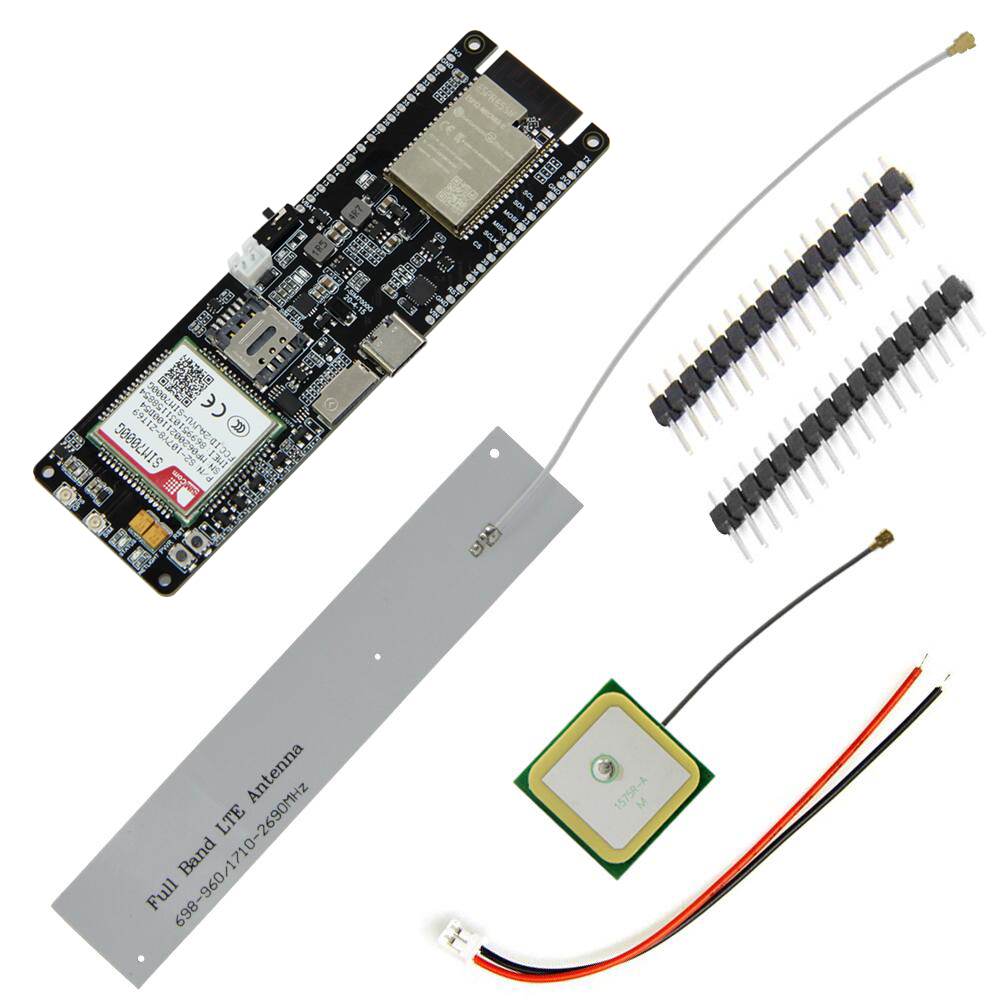
\includegraphics[width=\linewidth]{images/lilygo-tsim7000g.jpg}
  \caption{Placa de desarrollo LILYGO TTGO T-SIM7000G usada en el proyecto \cite{4269LILYGO}.}
  \label{fig:lilygo}
\end{figure}

En lo referente al conexionado con el coche, y en estrecha relación con el diseño 3D,
se buscó un conector hembra de \ac{OBD}--II que permitiese definir el \textit{pinout}
hacia la placa en este caso. Se valoraron distintas opciones, y una de las más
interesantes resultó la siguiente:

\begin{figure}[H]
  \centering
  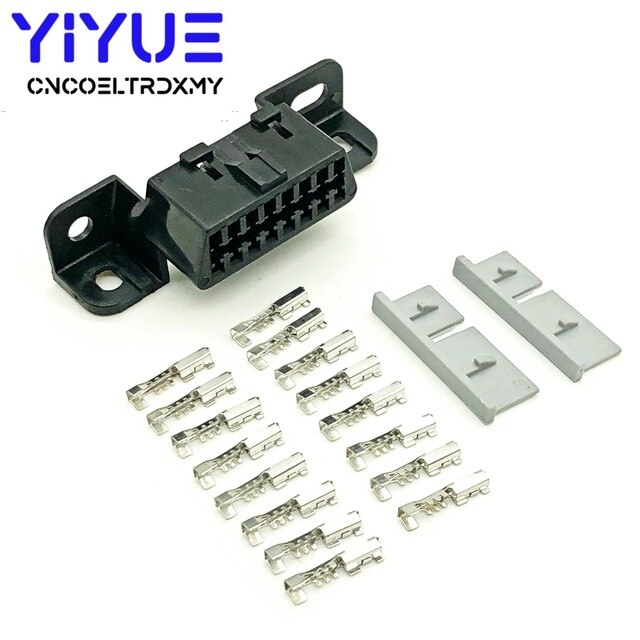
\includegraphics[width=\linewidth]{images/obd2-female.jpeg}
  \caption{Conector \ac{OBD}--II hembra con posibilidad de definir los pines de salida \cite{10DESCUENTOConector}.}
\end{figure}

También existen otros modelos que vienen ya configurados y que son más simples de
implementar, como:

\begin{figure}[H]
  \centering
  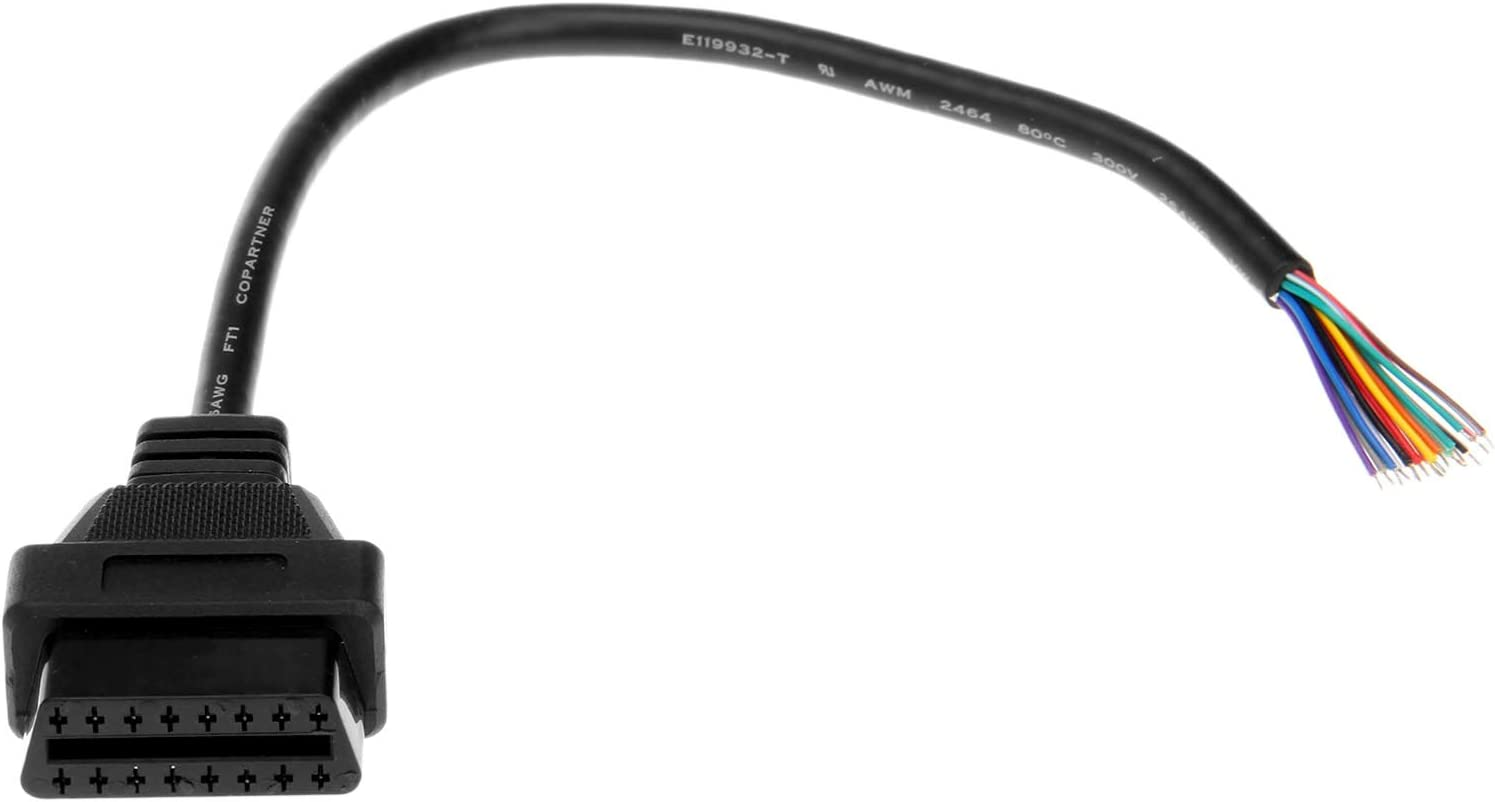
\includegraphics[width=\linewidth]{images/obd2-female-amazon.jpg}
  \caption{Conector \ac{OBD}--II hembra con cables ya incluidos \cite{AmazonComAupoko}.}
\end{figure}

Finalmente, para gestionar los sensores y conectores que necesita tener la placa para
funcionar correctamente, se diseñará una PCB que definirá la lógica de conexionado
para el correcto funcionamiento de todo el sistema al conjunto.
